\chapter{Общие уравнения симметрично-противоточного каскада}


\section{Понятие разделительного элемента, ступени, каскада.}


\subsection{Понятие разделительного элемента}

Газовая центрифуга




\subsection{Понятие разделительной ступени}

Ниже рассмотрены общие характеристики разделительных ступеней, предназначенных для разделения многокомпонентных изотопных смесей в газовой фазе. В качестве разделяемой изотопной смеси рассмотрена изотопная смесь, содержащая \textit{m} химически не реагирующих между собой компонентов, содержание которых будем определять их мольными долями (концентрациями) $C_{i}$ ($i=1,\, 2,...,m$) \cite{sulaberidzeTeoriyaKaskadovDlya2011}. Компоненты пронумерованы в порядке возрастания массовых чисел. Для концентраций компонентов разделяемой смеси справедливо очевидное тождество:

\begin{equation} \label{GrindEQ__1_1_} 
  \sum _{j=1}^{m}C_{j}  =1 
\end{equation} 
  
Как правило, вместо концентраций $C_{i} $, используют относительные концентрации, определяемые по отношению к концентрации так называемого «опорного» компонента с фиксированным номером, например, \textit{k}, то есть

\begin{equation} \label{GrindEQ__1_2_} 
  R_{ik} =\frac{C_{i} }{C_{k} } , i=1,\, 2,...,m.             
\end{equation} 
  
В качестве <<опорного>> может быть выбран любой из компонентов смеси, всего имеется   таких наборов. 
Простая разделительная ступень имеет один входной поток и два выходных (рис. \ref{1_1}). На вход ступени поступает поток питания (производительность ступени) $L$  (в моль/с) с концентрациями $C_{i}$ ($i=1,\, 2,...,m$). Из ступени выходят два потока: легкая фракция (поток, обогащенный легкими компонентами) или отбор ступени $L'$ и тяжелая фракция (поток, обедненный легкими компонентами) или отвал ступени $L''$. Концентрации компонентов в этих потоках  $C'_{i} $ и $C''_{i} $  соответственно.

\begin{figure}[ht]
  \centerfloat{\includegraphics[scale=0.7]{images/theory/lu15087t0po}}
  \caption{Схема разделительной ступени }\label{1_1}
\end{figure}

Коэффициент деления потоков смеси (срез) $\theta$, парциальные потоки компонентов $G_{i} ,\; G'_{i} ,\; G''_{i}$ и срезы парциальных потоков $\phi _{i}$ можно определить по формулам:

\begin{equation} \label{GrindEQ__1_3_} 
  \theta =\frac{L'}{L} ,\; G_{i} =LC_{i} ,\; G'_{i} =L'C'_{i} ,\; G''_{i} =L''C''_{i} , 
  \end{equation} 
  \begin{equation} \label{GrindEQ__1_4_} 
  \phi _{i} =\frac{G'_{i} }{G_{i} } ,\; 1-\phi _{i} =\frac{G"_{i} }{G_{i} } ,\; i=1,2,...,m. 
  \end{equation} 

Уравнения баланса ступени в стационарном режиме работы и в отсутствие потерь рабочего вещества имеют вид:

\begin{equation} \label{GrindEQ__1_5_} 
  L=L'+L'', 
  \end{equation} 
  \begin{equation} \label{GrindEQ__1_6_} 
  G_{i} =G'_{i} +G''_{i} , i=1,\, 2,...,m.             
\end{equation} 
  

Введенное в \ref{GrindEQ__1_3_} определение среза потоков ступени дает возможность представить уравнения \ref{GrindEQ__1_6_} в следующем виде:

\begin{equation} \label{GrindEQ__1_7_} 
  C_{i} =\theta C'_{i} +(1-\theta )C''_{i} . 
\end{equation} 

Из \ref{GrindEQ__1_5_} и \ref{GrindEQ__1_6_} непосредственно следует:

\begin{equation} \label{GrindEQ__1_8_} 
  L=\sum _{j=1}^{m}G_{j}  ,\; \; L'=\sum _{j=1}^{m}G'_{j} ,\; \;  L''=\sum _{j=1}^{m}G''_{j} ,\; \;   
  \end{equation} 
  \begin{equation} \label{GrindEQ__1_9_} 
  C_{i} =\frac{G_{i} }{\sum _{j=1}^{m}G_{j}  } ,\; \; C'_{i} =\frac{G'_{i} }{\sum _{j=1}^{m}G'_{j}  } ,\; \; C''_{i} =\frac{G''_{i} }{\sum _{j=1}^{m}G''_{j}  } , i=1,\, 2,...,m,             
  \end{equation} 
  \begin{equation} \label{GrindEQ__1_10_} 
  \theta =\frac{\sum _{j=1}^{m}G'_{j}  }{\sum _{j=1}^{m}G_{j}  } .            
\end{equation} 

Для каждого компонента $i$ с относительной концентрацией $R_{ik}$ вводят относительные коэффициенты разделения: полный $q_{ik}$, в отборе $\alpha _{ik} $ и в отвале $\beta _{ik} $ и соответствующие коэффициенты обогащения $\varepsilon _{ik} ,\varepsilon '_{ik} ,\; \varepsilon ''_{ik} \; $
\[q_{ik} =\frac{R'_{ik} }{R''_{ik} } ,\; \; \alpha _{ik} =\frac{R'_{ik} }{R_{ik} } ,\; \; \beta _{ik} =\frac{R_{ik} }{R''_{ik} } ,\] 

\begin{equation} \label{GrindEQ__1_11_} 
  \begin{array}{l}
    \qquad q_{i k}=\frac{R_{i k}^{\prime}}{R_{i k}^{\prime \prime}}, \alpha_{i k}=\frac{R_{i k}^{\prime}}{R_{i k}}, \beta_{i k}=\frac{R_{i k}}{R_{i k}^{\prime \prime}} \\
    \varepsilon_{i k}=q_{i k}-1, \varepsilon_{i k}^{\prime}=\alpha_{i k}-1, \varepsilon_{i k}^{\prime \prime}=1-\frac{1}{\beta_{i k}}
    \end{array}
\end{equation} 

При разделении изотопов молекулярно-кинетическими методами величины относительных коэффициентов разделения можно аппроксимировать соотношениями $q_{ij} =q_{0} {}^{M_{j} -M_{i} }$, где \textit{q}${}_{0}$ – коэффициент разделения, приходящийся на единицу разности массовых чисел; \textit{M${}_{i}$, M${}_{j}$} – массовые числа $i$-го и $j$-го компонентов, соответственно \cite{sulaberidzeTeoriyaKaskadovDlya2011}.

При фиксированном номере «опорного» компонента (в качестве «опорного» выбран компонент с номером $k$) существует набор из ($m-1$) независимых $q_{ik} $ (или $\alpha _{ik} $, $\beta _{ik}$). По определению $R_{ik} $ имеется $m$ таких наборов. Однако, каждый из них, например $q_{ik} $, может быть преобразован в другой набор, например, $q_{ij}$ по формулам

\begin{equation} \label{GrindEQ__1_12_} 
  q_{ij} =q_{ik} \cdot q_{kj} .            
\end{equation} 

Если $k\ne m$, то при всех $i<k$ значения всех коэффициентов разделения $q_{ik} $, $\alpha _{ik} $, $\beta _{ik} $, будут больше единицы, а при всех $i>k$ -- меньше единицы.

Полные коэффициенты разделения $q_{ik} $, как правило, не зависят от состава смеси. В некоторых случаях, что характерно для газовой центрифуги, коэффициенты $q_{ik} $ могут зависеть от коэффициента деления потоков смеси (срез) $\theta $. Так, в общем случае, для газовой центрифуги, полный коэффициент разделения зависит также от коэффициента деления потоков смеси (срез) $\theta$ и от потока питания на один разделительный элемент ступени $g_{s} $ (\ref{GrindEQ__q_}) \cite{mustafinObjectiveFunctionOptimization2019}:

\begin{equation} \label{GrindEQ__q_} 
  q_{ij} = f(\theta, g_{s}),              
\end{equation}

Далее будем рассматривать случай усредненной величины коэффициента разделения. Введем обозначения:

\begin{equation} \label{GrindEQ__1_13_} 
  g_{i} =\frac{\phi _{i} }{1-\phi _{i} } =\frac{G'_{i} }{G''_{i} } , i\ne k, 
  \end{equation} 
  \begin{equation} \label{GrindEQ__1_14_} 
  g_{k} =\frac{\phi _{k} }{1-\phi _{k} } =\frac{G'_{k} }{G''_{k} } .           
\end{equation} 

Нетрудно показать, используя  \ref{GrindEQ__1_9_} и  \ref{GrindEQ__1_11_}, что величины $g_{i}$ и $g_{k}$  связаны с величинами относительных коэффициентов разделения следующими соотношениями:

\begin{equation} \label{GrindEQ__1_15_} 
  g_{i} =\frac{\alpha _{ik} (\beta _{ik} -1)}{\alpha _{ik} -1} ,\; \; i\ne k,           
  \end{equation} 
  \begin{equation} \label{GrindEQ__1_16_} 
  g_{k} =\frac{\beta _{ik} -1}{(\alpha _{ik} -1)\beta _{ik} } =\frac{\varepsilon ''_{ik} }{\varepsilon '_{ik} } . 
\end{equation} 

При этом

\begin{equation} \label{GrindEQ__1_17_} 
  \frac{g_{i} }{g_{k} } =q_{ik} .           
\end{equation} 

\subsection{Понятие каскада}

С использованием выражений \ref{GrindEQ__1_1_}--\ref{GrindEQ__1_17_} получим следующие соотношения, связывающие параметры отдельной ступени каскада

\begin{equation} \label{GrindEQ__1_18_} 
  L=\sum _{j=1}^{m}L_{i}  =\sum _{j=1}^{m}\frac{g_{i} +1}{g_{i} }  L_{i} ',               
  \end{equation} 
  \begin{equation} \label{GrindEQ__1_19_} 
  C_{i} =\frac{g_{i} +1}{g_{i} } \frac{L_{i} '}{L} ,         
  \end{equation} 
  \begin{equation} \label{GrindEQ__1_20_} 
  \theta =\frac{L^{'} }{L} ={\sum _{j=1}^{m}L_{j}^{'}  \mathord{\left/ {\vphantom {\sum _{j=1}^{m}L_{j}^{'}   \sum _{j=1}^{m}L_{j}  }} \right. \kern-\nulldelimiterspace} \sum _{j=1}^{m}L_{j}  } .      
\end{equation} 



\section{Получение уравнений симметрично-противоточного каскада для случая произвольного числа компонентов и произвольных коэффициентов разделения.}


Среди различных способов коммутации ступеней в разделительных каскадах наиболее распространенным является так называемый способ симметричного соединения ступеней в противоточной схеме (рис. \ref{1_2}). Рассмотрим схему такого каскада, имеющего один входящий поток питания $F$ и два выходящих: отбор $P$, обогащенный самым легким компонентом и отвал W, обогащенный самым тяжелым компонентом. Потоки $F$, $P$, $W$ и концентрации компонентов в них $C_{i}^{F} ,\; \; C_{i}^{P} ,\; \; C_{i}^{W} \; \; (i=1,\; 2,...,m)$ являются внешними параметрами каскада. Следует заметить, что в случае разделения многокомпонентных смесей понятия «отбор» и «отвал» условны, поскольку ценный компонент может обогащаться как вместе с самым легким компонентом смеси, так и вместе с самым тяжелым.

\begin{figure}[ht]
  \centerfloat{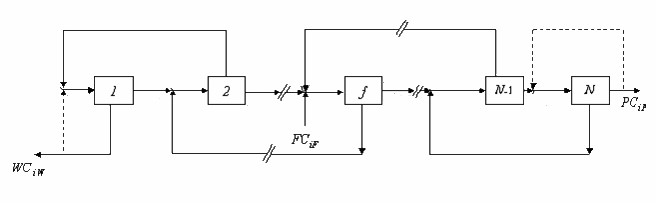
\includegraphics[scale=0.7]{images/theory/2}}
  \caption{Схема соединения ступеней в симметрично-противоточном каскаде}\label{1_2}
\end{figure}

В отсутствие потерь рабочего вещества на ступенях каскада, внешние параметры каскада должны удовлетворять уравнениям материального баланса

\begin{equation} \label{GrindEQ__1_21_} 
  \begin{array}{l} {\quad \quad \quad \quad F=P+W,} \\ {FC_{i}^{F} =PC_{i}^{P} +WC_{i}^{W} ,\; i=1,2,...,m.} \end{array} 
\end{equation} 

Ступени каскада пронумерованы последовательно от $s=1$ на отвальной ступени каскада до $s=N$ на отборной ступени. Считаем, что внешнее питание каскада (\textit{F}) подают на вход ступени с номером $f$. Внутренние параметры произвольной ступени с номером \textit{s} ($L_{s} $, $L'_{s} ,$ $L''_{s} ,$ $G_{i,s} ,$ $G'_{i,s} ,$ $G''_{i,s} $), где $L$ -- потоки вещества, а $G$ -- парциальные потоки (изотопов с индексами $i$) в стационарном режиме работы каскада, в отсутствие потерь рабочего вещества на ступенях каскада, согласно  \ref{GrindEQ__1_5_},  \ref{GrindEQ__1_6_} связаны уравнениями баланса вещества и каждого компонента

\begin{equation} \label{GrindEQ__1_22_} 
  L_{s} =L'_{s} +L''_{s} ,\; \; s=1,...,N,            
  \end{equation} 
  \begin{equation} \label{GrindEQ__1_23_} 
  G_{i,s} =G'_{i,s} +G''_{i,s} ,\;s=1,...,N \; i=1,2,...,m.           
  \end{equation} 

где индекс $i$ означает номер компонента.

Уравнения баланса в «узлах» (точках соединения межступенных потоков) при симметричном соединении ступеней имеют вид:

\begin{equation} \label{GrindEQ__1_24_} 
  L_{s} =\theta _{s-1} L_{s-1} +(1-\theta _{s+1} )L_{s+1} ,\; \; s=1,\, 2,...,f-1,\, f+1,...,N, 
  \end{equation} 
  \begin{equation} \label{GrindEQ__1_25_} 
  \begin{array}{l} {L_{s} C_{i,s} =\theta _{s-1} L_{s-1} C'_{i,s-1} +(1-\theta _{s+1} )L_{s+1} C''_{i,s+1} ,\; \; s=1,\, 2,...,f-1,\, f+1,...,N,} \\ {\; \; \; \; \; \; \; \; \; \; \; \; \; \; \; \; \; \; \; \; \; \; \; \; \; \; \; \; \; \; \; \; \; \quad \quad \quad \quad \quad \; \; \; \; \; \; \; \; \; \; \; \; \; \quad \quad \quad \; \; \; \; \; \; \; \; \; \; \; \; \; \quad \quad \quad \; \; \; \; \; \; \; \; \; \; \; \; \; \quad \quad \; \quad i=1,\, 2,...,m.} \end{array} 
  \end{equation} 

Для ступени подачи питания $f$ аналогичные уравнения выглядят так:

\begin{equation} \label{GrindEQ__1_26_} 
  L_{f} =\theta _{f-1} L_{f-1} +(1-\theta _{f+1} )L_{f+1} +F, 
  \end{equation} 
  \begin{equation} \label{GrindEQ__1_27_} 
  L_{f} C_{i,f} =\theta _{f-1} L_{f-1} C'_{i,f-1} +(1-\theta _{f+1} )L_{f+1} C''_{i,f+1} +FC_{i}^{F} ,\quad i=\overline{1,m}.            
\end{equation}

Внешние и внутренние параметры каскада связаны граничными условиями

\begin{equation} \label{GrindEQ__1_28_} 
  L_{0} =L'_{0} =L''_{0} =L_{N+1} =L'_{N+1} =L''_{N+1} =0, 
  \end{equation} 
  \begin{equation} \label{GrindEQ__1_29_} 
  L'_{N} =\theta _{N} L_{N} =P,        
  \end{equation} 
  \begin{equation} \label{GrindEQ__1_30_} 
  L''_{1} =(1-\theta _{1} )L_{1} =W,        
  \end{equation} 
  \begin{equation} \label{GrindEQ__1_31_} 
  C'_{N} =C_{i}^{P} ,\; i=1,\; \; 2,...,m, 
  \end{equation} 
  \begin{equation} \label{GrindEQ__1_32_} 
  C''_{1} =C_{i}^{W} ,\; i=1,\; \; 2,...,m, 
  \end{equation} 
  \begin{equation} \label{GrindEQ__1_33_} 
  G'_{i,N} =PC_{i}^{P} ,\; i=1,\; \; 2,...,m, 
  \end{equation} 
  \begin{equation} \label{GrindEQ__1_34_} 
  G''_{i,1} =WC_{i}^{W} ,\; i=1,\; \; 2,...,m. 
\end{equation} 

Соотношения (\ref{GrindEQ__1_21_})--(\ref{GrindEQ__1_34_}) описывают простейшую физико-математическую модель противоточного симметричного каскада, предназначенного для разделения многокомпонентной смеси. При решении некоторых разделительных задач вместо уравнений (\ref{GrindEQ__1_24_})--(\ref{GrindEQ__1_27_}) удобнее пользоваться разностными уравнениями, отражающими баланс потоков в сечениях между ступенями:

для обогатительной части каскада:

\begin{equation} \label{GrindEQ__1_35_} 
  \theta _{s} L_{s} -(1-\theta _{s+1} )L_{s+1} =P, 
  \end{equation} 
  \begin{equation} \label{GrindEQ__1_36_} 
  \theta _{s} L_{s} C'_{i,s} -(1-\theta _{s+1} )L_{s+1} C''_{i,s+1} =PC_{i}^{P} \; \; i=1,\, 2,...,m,        
  \end{equation} 

для обеднительной части каскада:

\begin{equation} \label{GrindEQ__1_37_} 
  \theta _{s} L_{s} -(1-\theta _{s+1} )L_{s+1} =-W, 
  \end{equation} 
  \begin{equation} \label{GrindEQ__1_38_} 
  \theta _{s} L_{s} C'_{i,s} -(1-\theta _{s+1} )L_{s+1} C''_{i,s+1} =-WC_{i}^{W} \; i=1,\; \; 2,...,\; m.        
  \end{equation} 

Величины, стоящие в левых частях уравнений (\ref{GrindEQ__1_35_})--(\ref{GrindEQ__1_38_}), как правило, называют «транзитными» потоками смеси в целом (уравнения (\ref{GrindEQ__1_35_}) и (\ref{GrindEQ__1_37_})) и ее отдельных компонентов (уравнения (\ref{GrindEQ__1_36_}) и (\ref{GrindEQ__1_38_})) \cite{sulaberidzeTeoriyaKaskadovDlya2011}. С физической точки зрения указанные уравнения определяют величину количества переносимого вещества в направлении от отвала к отбору. Отметим, что, в случае необходимости, аналогичные уравнения могут быть получены и для переноса вещества в направлении от отбора к отвалу. 
В свою очередь система (\ref{GrindEQ__1_35_})--(\ref{GrindEQ__1_38_}) может быть легко преобразована к виду:

\begin{equation} \label{GrindEQ__1_39_} 
  C_{i,s+1} -C_{i,s} =\frac{\theta _{s} L_{s} }{(1-\theta _{s+1} )L_{s+1} } \delta '_{i,s} +\delta ''_{i,s+1} -\frac{P\left(C_{i}^{P} -C_{i,s} \right)}{(1-\theta _{s+1} )L_{s+1} } ,        
  \end{equation} 

\[i=1,\, 2,...,m;\; \; s=f,...,N,\] 

, где $\delta '_{i,s} =C'_{i,s} -C_{i,s} $ -- функция, представляющая собой изменение концентрации $i$-го компонента в потоке обогащенной фракции $s$-й ступени; $\delta ''_{i,s} =C_{i,s} -C''_{i,s} $ – функция, представляющая собой изменение концентрации i-го компонента в потоке обедненной фракции $s$-й ступени.

Соответственно, система (\ref{GrindEQ__1_35_})--(\ref{GrindEQ__1_38_}) может быть представлена в виде

\begin{equation} \label{GrindEQ__1_40_} 
  C_{i,s+1} -C_{i,s} =\frac{\theta _{s} L_{s} }{(1-\theta _{s+1} )L_{s+1} } \delta '_{i,s} +\delta ''_{i,s+1} -\frac{W(C_{i,s} -C_{i}^{W} )}{(1-\theta _{s+1} )L_{s+1} } ,        
  \end{equation} 
  \[i=1,\, 2,...,m;\; \; s=1,\, 2,...,f-1.\] 

Отметим, что системы (\ref{GrindEQ__1_24_})--(\ref{GrindEQ__1_27_}), (\ref{GrindEQ__1_35_})--(\ref{GrindEQ__1_38_}) и (\ref{GrindEQ__1_39_})--(\ref{GrindEQ__1_40_}) эквивалентны. Анализ данных систем показывает, что они обе представляют собой системы нелинейных разностных уравнений относительно функций $C_{i,s}$. Существенной проблемой при решении подобных систем является то, что в эти уравнения (либо в их граничные условия) входят значения концентраций, которые неизвестны заранее и должны быть определены из решения этих же уравнений. Аналитическое решение подобных систем удается найти лишь для некоторых частных случаев (данные случаи рассмотрены ниже) \cite{sulaberidzeTeoriyaKaskadovDlya2011}. В общем случае, системы (\ref{GrindEQ__1_24_})--(\ref{GrindEQ__1_27_}), (\ref{GrindEQ__1_35_})--(\ref{GrindEQ__1_38_}) или (\ref{GrindEQ__1_39_})--(\ref{GrindEQ__1_40_}) требуют использования численных методов. При этом, как правило, выделяют 2 типа задач расчета параметров каскада: поверочный расчет и проектировочный расчет.

Под поверочным расчетом каскада подразумевают следующую задачу:
Задано: состав исходной разделяемой смеси,  число ступеней в каскаде и величины питающих их потоков, величины внешнего потока питания и одного из выходящих потоков каскада (отбора или отвала), параметры ступени (например, относительные коэффициенты разделения ступеней и др.).
Подлежат определению: концентрации всех компонентов в потоках отбора  и отвала и распределение концентраций компонентов по ступеням каскада. 
Поверочный расчет каскада необходим при исследовании оптимального управления процессом разделения, при изменении режимов работы и отдельных параметров разделительного каскада \cite{sulaberidzeTeoriyaKaskadovDlya2011}. Основные трудности поверочного расчета связаны с тем, что неизвестные концентрации компонентов в потоках отбора и отвала сами явно входят в основные уравнения переноса (или их граничные условия). Невозможность аналитического решения этих уравнений вызывает необходимость разработки численных методов, малочувствительных к заданию начальных приближений для концентраций компонентов в выходящих потоках. На сегодняшний день предложены различные методы поверочного расчета, которые позволяют численно решить данную задачу \cite{sulaberidzeTeoriyaKaskadovDlya2011, sazykinUsovershenstvovannyyMetodRascheta1997, wuCalculationMethodsDetermining1988, holpanovEffektivnyyMetodRascheta1998, potapovCalculationSquaredoffCascades1996, zengRobustEfficientCalculation2000}.

Под проектировочным расчетом каскада обычно подразумевают следующую задачу \cite{sulaberidzeTeoriyaKaskadovDlya2011}.
Задано: состав исходной разделяемой смеси, один из выходящих потоков каскада (отбор или отвал), концентрации одного из компонентов (целевого или ключевого) в потоках отбора и отвала.
Подлежат определению: все внутренние параметры каскада (распределение потока и концентраций компонентов по ступеням каскада и др.), концентрации остальных компонентов (всех кроме ключевого) в потоках отбора и отвала. 
При этом, очевидно, что найденные параметры каскада должны соответствовать оптимальным условиям разделения в каскаде.
